%╔════════════════════════════╗
%║	  Szablon dostosował	  ║
%║	mgr inż. Dawid Kotlarski  ║
%║		  06.10.2024		  ║
%╚════════════════════════════╝
\documentclass[12pt,twoside,a4paper,openany]{article}

    % ------------------------------------------------------------------------
% PAKIETY
% ------------------------------------------------------------------------

%różne pakiety matematyczne, warto przejrzeć dokumentację, muszą być powyżej ustawień językowych.
\usepackage{mathrsfs}   %Różne symbole matematyczne opisane w katalogu ~\doc\latex\comprehensive. Zamienia \mathcal{L} ze zwykłego L na L-transformatę.
\usepackage{eucal}      %Różne symbole matematyczne.
\usepackage{amssymb}    %Różne symbole matematyczne.
\usepackage{amsmath}    %Dodatkowe funkcje matematyczne, np. polecenie \dfac{}{} skladajace ulamek w trybie wystawionym (porównaj $\dfrac{1}{2}$, a $\frac{1}{2}$).

%język polski i klawiatura
\usepackage[polish]{babel}
%\usepackage{qtimes} % czcionka Times new Roman
\usepackage[OT4]{polski}
%\usepackage[cp1250]{inputenc}                       %Strona kodowa polskich znaków.

%obsługa pdf'a
\usepackage[pdftex,usenames,dvipsnames]{color}      %Obsługa kolorów. Opcje usenames i dvipsnames wprowadzają dodatkowe nazwy kolorow.
\usepackage[pdftex,pagebackref=false,draft=false,pdfpagelabels=false,colorlinks=true,urlcolor=blue,linkcolor=black,citecolor=green,pdfstartview=FitH,pdfstartpage=1,pdfpagemode=UseOutlines,bookmarks=true,bookmarksopen=true,bookmarksopenlevel=2,bookmarksnumbered=true,pdfauthor={Dawid Kotlarski},pdftitle={Dokumentacja Projektowa},pdfsubject={},pdfkeywords={transient recovery voltage trv},unicode=true]{hyperref}   %Opcja pagebackref=true dotyczy bibliografii: pokazuje w spisie literatury numery stron, na których odwołano się do danej pozycji.

%bibliografia
%\usepackage[numbers,sort&compress]{natbib}  %Porządkuje zawartość odnośników do literatury, np. [2-4,6]. Musi być pod pdf'em, a styl bibliogfafii musi mieć nazwę z dodatkiem 'nat', np. \bibliographystyle{unsrtnat} (w kolejności cytowania).
\usepackage[
backend=biber,
style=numeric,
sorting=none
]{biblatex}
\addbibresource{bibliografia.bib}
\usepackage{hypernat}                       %Potrzebna pakietowi natbib do wspolpracy z pakietem hyperref (wazna kolejnosc: 1. hyperref, 2. natbib, 3. hypernat).

%grafika i geometria strony
\usepackage{extsizes}           %Dostepne inne rozmiary czcionek, np. 14 w poleceniu: \documentclass[14pt]{article}.
\usepackage[final]{graphicx}
\usepackage[a4paper,left=3.5cm,right=2.5cm,top=2.5cm,bottom=2.5cm]{geometry}

%strona tytułowa
\usepackage{strona_tytulowa}

%inne
\usepackage[hide]{todo}                     %Wprowadza polecenie \todo{treść}. Opcje pakietu: hide/show. Polecenie \todos ma byc na koncu dokumentu, wszystkie \todo{} po \todos sa ignorowane.
\usepackage[basic,physics]{circ}            %Wprowadza środowisko circuit do rysowania obwodów elektrycznych. Musi byc poniżej pakietow językowych.
\usepackage[sf,bf,outermarks]{titlesec}     %Troszczy się o wygląd tytułów rozdziałów (section, subsection, ...). sf oznacza czcionkę sans serif (typu arial), bf -- bold. U mnie: oddzielna linia dla naglowku paragraph. Patrz tez: tocloft -- lepiej robi format spisu tresci.
\usepackage{tocloft}                        %Troszczy się o format spisu trsci.
\usepackage{expdlist}    %Zmienia definicję środowiska description, daje większe możliwości wpływu na wygląd listy.
\usepackage{flafter}     %Wprowadza parametr [tb] do polecenia \suppressfloats[t] (polecenie to powoduje nie umieszczanie rysunkow, tabel itp. na stronach, na ktorych jest to polecenie (np. moze byc to stroma z tytulem rozdzialu, ktory chcemy zeby byl u samej gory, a nie np. pod rysunkiem)).
\usepackage{array}       %Ładniej drukuje tabelki (np. daje wiecej miejsca w komorkach -- nie są tak ścieśnione, jak bez tego pakietu).
\usepackage{listings}    %Listingi programow.
\usepackage[format=hang,labelsep=period,labelfont={bf,small},textfont=small]{caption}   %Formatuje podpisy pod rysunkami i tabelami. Parametr 'hang' powoduje wcięcie kolejnych linii podpisu na szerokosc nazwy podpisu, np. 'Rysunek 1.'.
\usepackage{appendix}    %Troszczy się o załączniki.
\usepackage{floatflt}    %Troszczy się o oblewanie rysunkow tekstem.
\usepackage{here}        %Wprowadza dodtkowy parametr umiejscowienia rysunków, tabel, itp.: H (duże). Umiejscawia obiekty ruchome dokladnie tam gdzie są w kodzie źródłowym dokumentu.
\usepackage{makeidx}     %Troszczy się o indeks (skorowidz).

%nieużywane, ale potencjalnie przydatne
\usepackage{sectsty}           %Formatuje nagłówki, np. żeby były kolorowe -- polecenie: \allsectionsfont{\color{Blue}}.
%\usepackage{version}           %Wersje dokumentu.

%============
\usepackage{longtable}			%tabelka
%============

%============
% Ustawienia listingów do kodu
%============

\usepackage{listings}
\usepackage{xcolor}

\definecolor{codegreen}{rgb}{0,0.6,0}
\definecolor{codegray}{rgb}{0.5,0.5,0.5}
\definecolor{codepurple}{rgb}{0.58,0,0.82}
\definecolor{backcolour}{rgb}{0.95,0.95,0.92}

% Definicja stylu "mystyle"
\lstdefinestyle{mystyle}{
	backgroundcolor=\color{backcolour},   
	commentstyle=\color{codegreen},
	keywordstyle=\color{blue},	%magenta
	numberstyle=\tiny\color{codegray},
	stringstyle=\color{codepurple},
	basicstyle=\ttfamily\footnotesize,
	breakatwhitespace=false,         
	breaklines=true,                 
	captionpos=b,                    
	keepspaces=true,                 
	numbers=left,                    
	numbersep=5pt,                  
	showspaces=false,                
	showstringspaces=false,
	showtabs=false,                  
	tabsize=2
}

\lstset{style=mystyle} % Deklaracja aktywnego stylu
%===========

%PAGINA GÓRNA I DOLNA
\usepackage{fancyhdr}          %Dodaje naglowki jakie się chce.
\pagestyle{fancy}
\fancyhf{}
% numery stron w paginie dolnej na srodku
\fancyfoot[C]{\scriptsize DOKUMENTACJA PROJEKTU - ZAAWANSOWANE PROGRAMOWANIE \\ 
\normalsize\sffamily  \thepage}


%\fancyhead[L]{\small\sffamily \nouppercase{\leftmark}}
\fancyhead[C]{\footnotesize \textit{AKADEMIA NAUK STOSOWANYCH W NOWYM SĄCZU}\\}

\renewcommand{\headrulewidth}{0.4pt}
\renewcommand{\footrulewidth}{0.4pt}

    % ------------------------------------------------------------------------
% USTAWIENIA
% ------------------------------------------------------------------------

% ------------------------------------------------------------------------
%   Kropki po numerach sekcji, podsekcji, itd.
%   Np. 1.2. Tytuł podrozdziału
% ------------------------------------------------------------------------
\makeatletter
    \def\numberline#1{\hb@xt@\@tempdima{#1.\hfil}}                      %kropki w spisie treści
    \renewcommand*\@seccntformat[1]{\csname the#1\endcsname.\enspace}   %kropki w treści dokumentu
\makeatother

% ------------------------------------------------------------------------
%   Numeracja równań, rysunków i tabel
%   Np.: (1.2), gdzie:
%   1 - numer sekcji, 2 - numer równania, rysunku, tabeli
%   Uwaga ogólna: o otoczeniu figure ma być najpierw \caption{}, potem \label{}, inaczej odnośnik nie działa!
% ------------------------------------------------------------------------
\makeatletter
    \@addtoreset{equation}{section} %resetuje licznik po rozpoczęciu nowej sekcji
    \renewcommand{\theequation}{{\thesection}.\@arabic\c@equation} %dodaje kropki

    \@addtoreset{figure}{section}
    \renewcommand{\thefigure}{{\thesection}.\@arabic\c@figure}

    \@addtoreset{table}{section}
    \renewcommand{\thetable}{{\thesection}.\@arabic\c@table}
\makeatother

% ------------------------------------------------------------------------
% Tablica
% ------------------------------------------------------------------------
\newenvironment{tabela}[3]
{
    \begin{table}[!htb]
    \centering
    \caption[#1]{#2}
    \vskip 9pt
    #3
}{
    \end{table}
}

% ------------------------------------------------------------------------
% Dostosowanie wyglądu pozycji listy \todos, np. zamiast 'p.' jest 'str.'
% ------------------------------------------------------------------------
\renewcommand{\todoitem}[2]{%
    \item \label{todo:\thetodo}%
    \ifx#1\todomark%
        \else\textbf{#1 }%
    \fi%
    (str.~\pageref{todopage:\thetodo})\ #2}
\renewcommand{\todoname}{Do zrobienia...}
\renewcommand{\todomark}{~uzupełnić}

% ------------------------------------------------------------------------
% Definicje
% ------------------------------------------------------------------------
\def\nonumsection#1{%
    \section*{#1}%
    \addcontentsline{toc}{section}{#1}%
    }
\def\nonumsubsection#1{%
    \subsection*{#1}%
    \addcontentsline{toc}{subsection}{#1}%
    }
\reversemarginpar %umieszcza notki po lewej stronie, czyli tam gdzie jest więcej miejsca
\def\notka#1{%
    \marginpar{\footnotesize{#1}}%
    }
\def\mathcal#1{%
    \mathscr{#1}%
    }
\newcommand{\atp}{ATP/EMTP} % Inaczej: \def\atp{ATP/EMTP}

% ------------------------------------------------------------------------
% Inne
% ------------------------------------------------------------------------
\frenchspacing                      
\hyphenation{ATP/-EMTP}             %dzielenie wyrazu w danym miejscu
\setlength{\parskip}{3pt}           %odstęp pomiędzy akapitami
\linespread{1.3}                    %odstęp pomiędzy liniami (interlinia)
\setcounter{tocdepth}{4}            %uwzględnianie w spisie treści czterech poziomów sekcji
\setcounter{secnumdepth}{4}         %numerowanie do czwartego poziomu sekcji 
\titleformat{\paragraph}[hang]      %wygląd nagłówków
{\normalfont\sffamily\bfseries}{\theparagraph}{1em}{}



    %polecenia zdefiniowane w pakiecie strona_tytulowa.sty
    \title{Algorytm Merge Sort oraz Demonstracja Unit Testów przy użyciu Google Test}		%...Wpisać nazwę projektu...
    \author{Mateusz Stanek}
    \authorII{}		%jeśli są dwie osoby w projekcie to zostawiamy:    \authorII{}
		
	\uczelnia{AKADEMIA NAUK STOSOWANYCH \\W NOWYM SĄCZU}
    \instytut{Wydział Nauk Inżynieryjnych}
    \kierunek{Katedra Informatyki}
    \praca{DOKUMENTACJA PROJEKTOWA}
    \przedmiot{ZAAWANSOWANE PROGRAMOWANIE}
    \prowadzacy{mgr inż. Dawid Kotlarski}
    \rok{2024}


%definicja składni mikrotik
\usepackage{fancyvrb}
\DefineVerbatimEnvironment{MT}{Verbatim}%
{commandchars=\+\[\],fontsize=\small,formatcom=\color{red},frame=lines,baselinestretch=1,} 
\let\mt\verb 
%zakonczenie definicji składni mikrotik

\usepackage{fancyhdr}    %biblioteka do nagłówka i stopki

			
\begin{document}
   
    \renewcommand{\figurename}{Rys.}    %musi byc pod \begin{document}, bo w~tym miejscu pakiet 'babel' narzuca swoje ustawienia
    \renewcommand{\tablename}{Tab.}     %j.w.
    \thispagestyle{empty}               %na tej stronie: brak numeru
    \stronatytulowa                     %strona tytułowa tworzona przez pakiet strona_tytulowa.tex
 
 \pagestyle{fancy}

    \newpage

    %formatowanie spisu treści i~nagłówków
    \renewcommand{\cftbeforesecskip}{8pt}
    \renewcommand{\cftsecafterpnum}{\vskip 8pt}
    \renewcommand{\cftparskip}{3pt}
    \renewcommand{\cfttoctitlefont}{\Large\bfseries\sffamily}
    \renewcommand{\cftsecfont}{\bfseries\sffamily}
    \renewcommand{\cftsubsecfont}{\sffamily}
    \renewcommand{\cftsubsubsecfont}{\sffamily}
    \renewcommand{\cftparafont}{\sffamily}
    %koniec formatowania spisu treści i nagłówków
     
    \tableofcontents    %spis treści
    \thispagestyle{fancy}
    \newpage

    
    \newpage

    
%%%%%%%%%%%%%%%%%%% treść główna dokumentu %%%%%%%%%%%%%%%%%%%%%%%%%

   	\newpage
\section{Ogólne określenie wymagań}		%1
%Określenie celu pracy, co chcemy uzyskać, jakie przewidujemy wyniki

\hspace{0.60cm}

Celem projektu jest stworzenie programu pozwalającego sortować tablicę algorytmem Merge Sort oraz kontrolowanie jego wersji za pomocą narzędzia git. Należy także stworzyć szereg unit testów mających na celu sprawdzenie poprawności programu. 

Program będzie podzielony na plik klasy, oraz plik zajmujący się testami.

Wynikiem projektu powinno być repozytorium git i działająca klasa sortująca tablicę oraz zbiór testów, które program spełnia.

   \newpage
\section{Analiza problemu}		%2
%Napisać gdzie używa się tego algorytmu
%Opisać sposób działania programu/algorytmu
%Napisać spsoób wykorzystania algorytmu po przez wykonanie przykładu (np. mnożenie macierzy - wykonać ręcznie przykład z mnożeniem macierzy pokazujący jak mnoży się macierz ręcznie)
%Jeśli zadanie zakłada przedstawienie jakiegoś narzędzia (np. git, AI) należy opisać narzędzie

\subsection{Algorytm Merge Sort}

Algorytm Merge Sort\cite{mergewiki} (Sortowanie przez Scalanie), jest algorytmem sortowania typu dziel i zwyciężaj\cite{divideandconquerwiki} o złożoności obliczeniowej najgorszego i średniego przypadku $ O(n \log{n}) $. Złożoność pamięciowa algorytmu wynosi natomiast $ O(n) $.

Algorytm polega na początkowym podzieleniu tablicy na jednoelementowe części. Następnie, części te są ze sobą stopniowo scalane. Przy scalaniu element jednej podtablicy porównywany jest z drugą. Mniejszy wynik porównania trafia do następnego "poziomu" scalonej tablicy, a algorytm przechodzi do porównywania następnego elementu danej podtablicy.

Graficzna reprezentacja algorytmu jest zaprezentowana na rysunku \ref{fig:mergesort}

\begin{figure}[H]
	\centering
	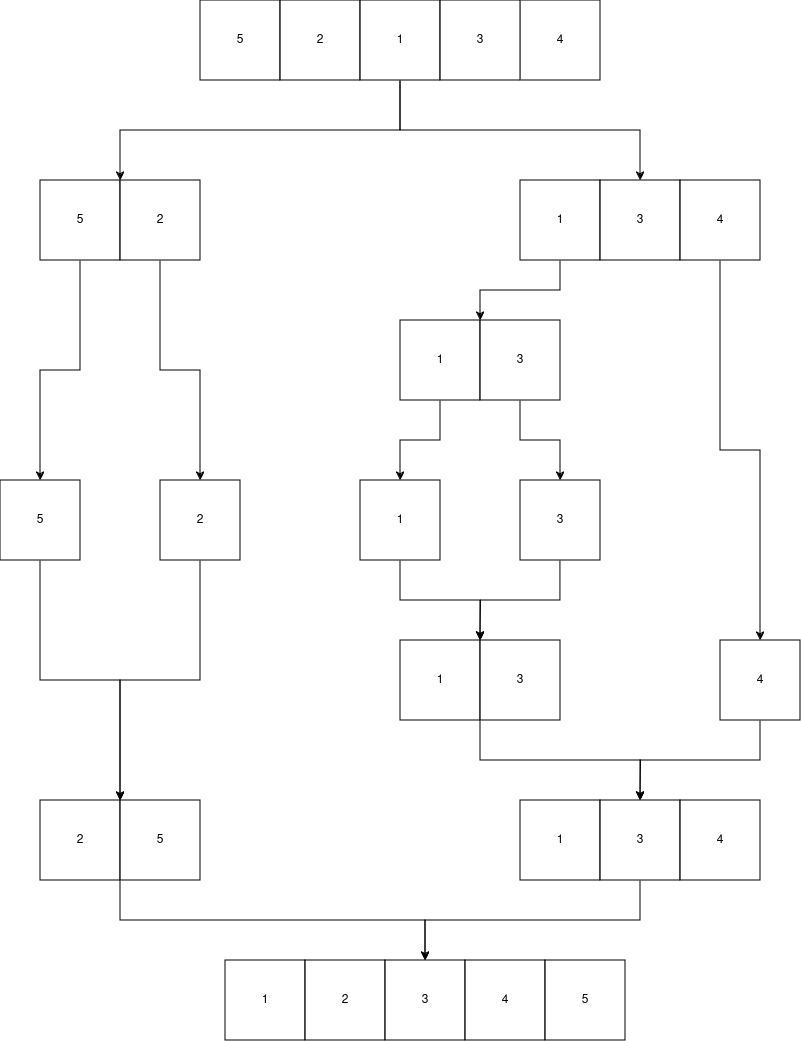
\includegraphics[width=0.7\linewidth]{images/mergesort.drawio.png}
	\caption{Reprezentacja sortowania Merge Sort}
	\label{fig:mergesort}
\end{figure}

\subsection{Git}
Kolejnym konceptem, którym zajmuje się projekt jest narzędzie git\cite{gitsite}. Pozwala ono zarządzać poszczególnymi wersjami projektów. Głównym korzeniem gita jest system commitów, czyli zapisania zmian w pliku w stosunku do commita starszego. To, w połączeniu z jego innymi możliwościami pozwala na tworzenie długich i skomplikowanych osi czasu danych projektów. 

Użycie gita można zademonstrować na prostym przykładzie. Tworzymy katalog a w nim repozytorium, uzywając komendy \texttt{git init}, jak widać na rys. \ref{fig:git_init}.

\begin{figure}[H]
	\centering
	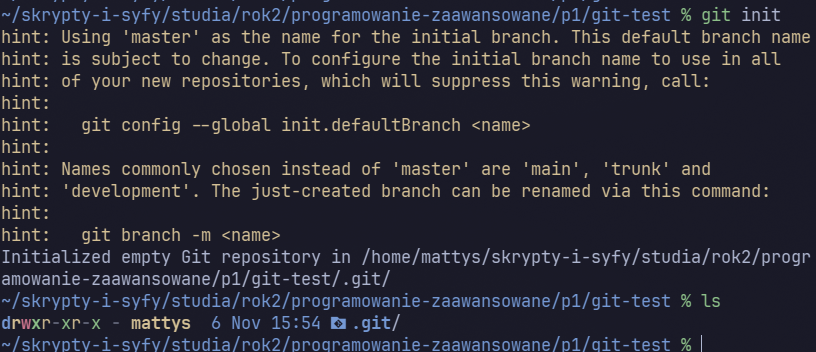
\includegraphics[width=1\textwidth]{images/git_init.png}
	\caption{\centering{Puste repozytorium git}}
	\label{fig:git_init}
\end{figure}

Stwórzmy jakiś plik i dodajmy go do repozytorium. Plik można dodać do repozytorium komendą \texttt{git add}

\begin{figure}[H]
	\centering
	
\includegraphics[width=1\textwidth]{images/git_add.png}
	\caption{\centering{Stworznie pliku w repozytorium}}
	\label{fig:git_add}
\end{figure}

Następnie należy scommitować zmiany. 

\begin{figure}[H]
	\centering
	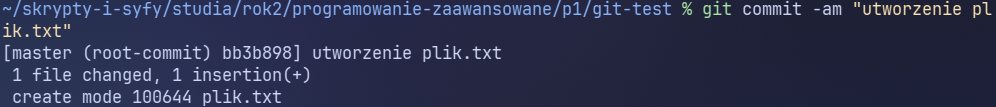
\includegraphics[width=1\textwidth]{images/git_commit1.png}
	\caption{\centering{Commit nr. 1}}
	\label{fig:git_commit1}
\end{figure}

Na rysunku \ref{fig:git_commit1} użyta komenda \texttt{git commit} commituje wszystkie dodane pliki (\texttt{-a}) z jakimś komunikatem (\texttt{-m}).  

\begin{figure}[H]
	\centering
	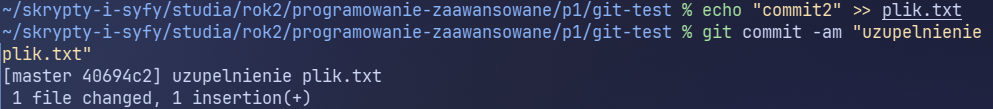
\includegraphics[width=1\textwidth]{images/git_commit2.png}
	\caption{\centering{Commit nr. 2}}
	\label{fig:git_commit2}
\end{figure}

Na rys. \ref{fig:git_commit2}, został utworzony kolejny commit, dodajacy zmiany do \texttt{plik.txt}.

\begin{figure}[H]
	\centering
	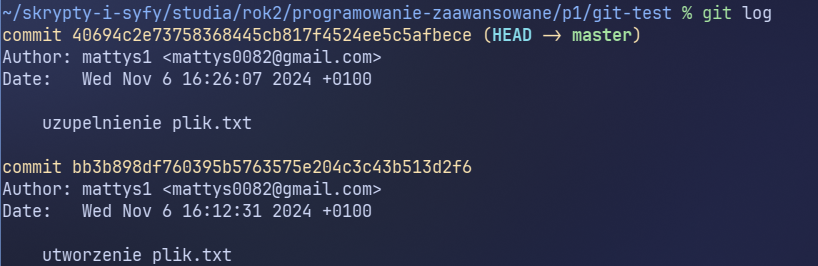
\includegraphics[width=1\textwidth]{images/git_log.png}
	\caption{\centering{Log gita}}
	\label{fig:git_log}
\end{figure}

Jak na rys. \ref{fig:git_log} jest pokazane, używając komendy \texttt{git log}, można wyświetlić log commitów w repozytorium.

\begin{figure}[H]
	\centering
	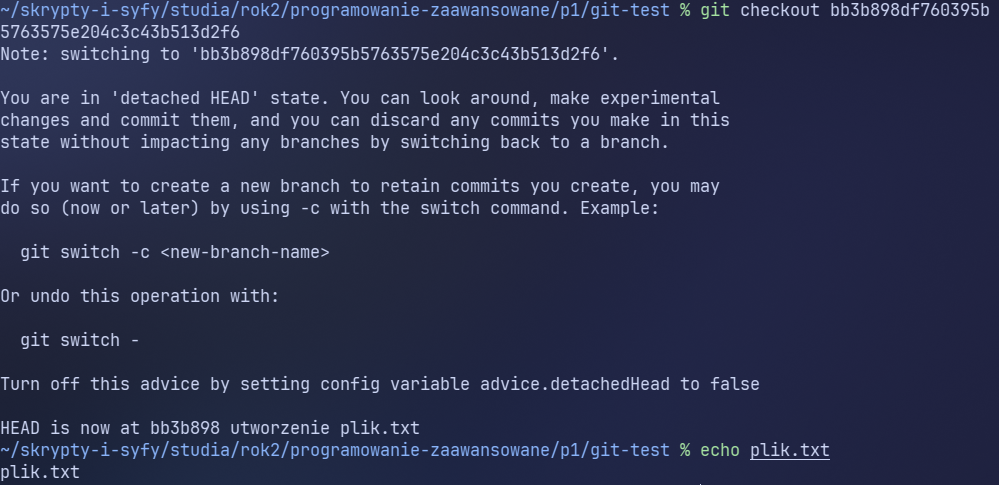
\includegraphics[width=1\textwidth]{images/git_checkout.png}
	\caption{\centering{Demonstracja checkout}}
	\label{fig:git_checkout}
\end{figure}

Jak widać na rys. \ref{fig:git_checkout}, komenda \texttt{git checkout}, pozwala na przejście repozytorium w inny stan, w tym przypadku przechodzi się do commita o danym ID, pokazanym na rys. \ref{fig:git_log}. Jako, że jest to pierwszy commit, nie ma w nim zmian z drugiego.

\subsection{Doxygen}
Doxygen\cite{doxygensite} jest narzędziem automatycznie generującym dokumentację programu z komentarzy w kodzie źródłowym. Potrafi on generować strony HTML, gdzie można dynamicznie nawigować się miedzy rożnymi częściami kodu oraz pliki \LaTeX, które można konwertować na różne, statyczne formaty.

\subsection{Google Test}
Google Test \cite{gtestrepo} jest frameworkiem stworzonym przez Google służącym do prowadzenia Unit Testów w języku \texttt{C++}. Narzędzie to pozwala na gwarantowanie poprawności logiki kodu.

   	\newpage
\section{Projektowanie}		%3
%Napisać z jakich narzędzi będziemy korzystać (kompilator, język programowania), git, biblioteki dodatkowe, itp.
%Opisać szczegółowe ustawienia kompilatora (jeśli są), powiązania z bibliotekami, itp.
%Narysować graf, UML, diagram klas, schemat działania algorytmu
%Jeśli zadanie zakłada przedstawienie jakiegoś narzędzia (np. git, AI) należy opisać sposób jego używania

\subsection{Implementacja Merge Sort}


Do zaimplementowania Merge Sorta zostanie użyty Język \texttt{C++} z kompilatorem \texttt{g++}. Wersja standardu \texttt{C++} to \texttt{C++20}. Jako, że projekt ma być rozdzielony na dwa pliki, zostanie zastosowany \texttt{CMake} w celu automatyzacji procesu budowania. \texttt{CMake} pozwala na generowanie plików budujących dany projekt, zgodnie z określoną konfiguracją. Oszczędza to programiście, szczególnie przy większych projektach, manualne pisanie Makefileów.
Plik konfiguracyjny \texttt{CMakeLists.txt} może wyglądać jak na rysunku

\begin{lstlisting}[caption=Plik konfiguracyjny CMake, label={lst:cmakelists}, language=C++]
	cmake_minimum_required(VERSION 3.15)
	
	set(PROJECT_NAME proj1)
	
	project(${PROJECT_NAME} VERSION 0.1 LANGUAGES CXX)
	
	set(CMAKE_CXX_STANDARD 20)
	set(CMAKE_CXX_STANDARD_REQUIRED ON)
	set(CMAKE_EXPORT_COMPILE_COMMANDS True)
	set(CMAKE_RUNTIME_OUTPUT_DIRECTORY ${CMAKE_CURRENT_LIST_DIR}/out)
	
	add_subdirectory(src)
	
\end{lstlisting}

Edytorem będzie program Neovim. Jest to terminalowy edytor tekstu z możliwością poszerzenia funkcjonalności przy użyciu wszelkiego rodzaju pluginów. Wybrany został, dlatego że jest on już skonfigurowany na moim komputerze zgodnie z moimi preferencjami.

\subsection{Git}

Dla ułatwienia pracy, zastosowany został front-end dla gita o nazwie lazygit. Jest to terminalowy program, którego główną zaletą jest łatwa nawigacja przy użyciu klawiatury. Ponadto, jest on lekki i szybki.

\subsection{Doxygen}

Konfiguracja dla Doxygena jest wygenerowana przy użyciu programu doxywizard, pokazany na rys. \ref{fig:doxywizard}, pozwalającego na graficzne zmienianie ustawień. Po wygenerowaniu konfiguracji, Doxygen wywoływany jest przy użyciu komendy.

\begin{figure}[H]
	\centering
	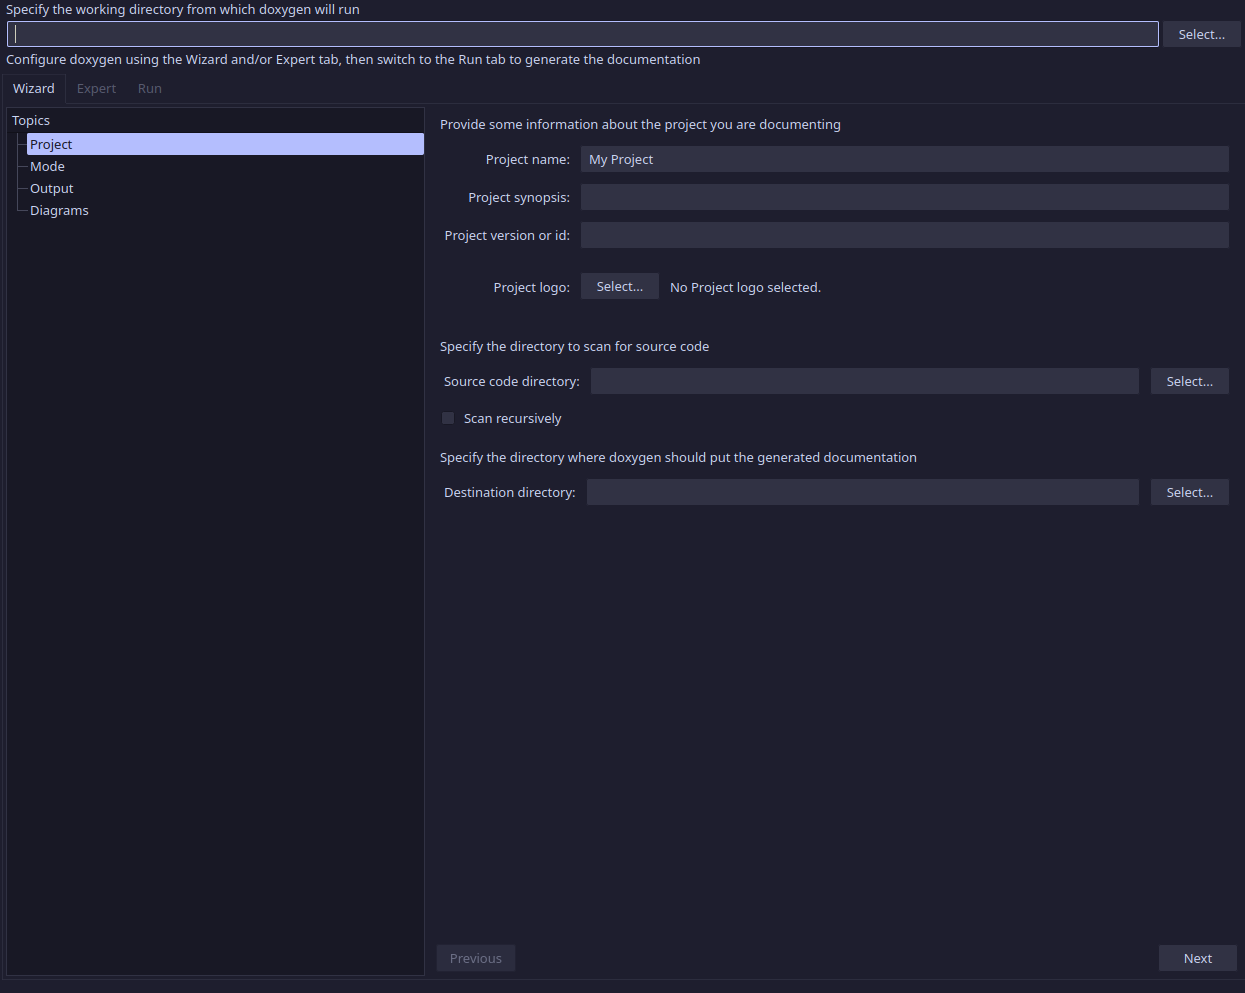
\includegraphics[width=1\textwidth]{images/doxywizard.png}
	\caption{\centering{Interfejs programu doxywizard}}
	\label{fig:doxywizard}
\end{figure}

\subsection{Google Test}

Google Test został dodany do projektu jako biblioteka w \texttt{CMake}, co zostało ukazane na listingu nr.~\ref{lst:gtestcmake}. Framework jest automatycznie pobierany i instalowany przy konfiguracji.

\begin{lstlisting}[caption=Dodanie Google Test do projektu, label={lst:gtestcmake}, language=C++]
include(FetchContent)
	FetchContent_Declare(
			googletest
			URL https://github.com/google/googletest/archive03597a01ee50ed33e9dfd640b249b4be3799d395.zip
	)
FetchContent_MakeAvailable(googletest)

\end{lstlisting}

Pliki źródłowe testów znajdują się we własnym folderze, więc też trzeba do niego dodać \texttt{CMakeLists}, jak widać na listingu nr.~\ref{lst:testscmake}

\begin{lstlisting}[caption=Dodanie Google Test do projektu, label={lst:testscmake}, language=C++]
file(GLOB_RECURSE SRC_FILES *.cpp *.h)
set(TESTS_EXECUTABLE ${PROJECT_NAME}_tests)

enable_testing()

add_executable(${TESTS_EXECUTABLE} ${SRC_FILES})

target_link_libraries(
	${TESTS_EXECUTABLE} PUBLIC
	${PROJECT_NAME}_lib
	GTest::gtest_main
)

\end{lstlisting}

Plik wykonywalny testów jest linkowany do - oprócz samego frameworka - biblioteki jaka jest wygenerowana z klasy \texttt{MergeSorter}, o której więcej w sekcji nr.~\ref{sec:MergeSorter}.

   	\newpage
\section{Implementacja}		%4
%Opisać implementacje algorytmu/programu. Pokazać ciekawe fragmenty kodu
%Opisać powstałe wyniki (algorytmu/nrzędzia)

\subsection{Klasa MergeSorter} \label{sec:MergeSorter}

Klasa jest zaimplementowana jako jeden plik \texttt{.hpp}. Nie jest podzielona na plik implementacji oraz nagłówek, ponieważ jest ona szablonem. Deklaracja klasy oraz prywatne elementy wyglądają tak jak na listingu nr.~\ref{lst:mergesorter}.

\begin{lstlisting}[caption=Klasa \texttt{MergeSorter}, label={lst:mergesorter}, language=C++]
template<typename T>
class MergeSorter {
private: 
	std::vector<T> mergeSort(const std::vector<T>& toMerge) {
		if(toMerge.size() <= 1) {
			return toMerge;
		}

		auto left = toMerge | std::views::take(toMerge.size() / 2) | std::ranges::to<std::vector>();
		auto right = toMerge | std::views::drop(toMerge.size() / 2) | std::ranges::to<std::vector>();

		auto sortedLeft = mergeSort(left);
		auto sortedRight = mergeSort(right);

		return merge(sortedLeft, sortedRight);
	}

	std::vector<T> merge(const std::vector<T>& left, const std::vector<T>& right) {
		std::vector<T> merged;
		auto leftIt { left.begin() }, rightIt { right.begin() };

		for (; leftIt != left.end() && rightIt != right.end();) {
			if(*leftIt <= *rightIt) {
				merged.push_back(*leftIt);
				leftIt++;
			} else {
				merged.push_back(*rightIt);
				rightIt++;
			}
		}

		merged.insert(merged.end(), leftIt, left.end());
		merged.insert(merged.end(), rightIt, right.end());
		
		return merged;
	}

public:
	void operator()(std::vector<T>& toSort) {
		if(toSort.size() <= 1) {
			return;
		}

		toSort = mergeSort(toSort);	
	}
};
\end{lstlisting}
  
Klasa posiada tylko jedną publiczną metodę, którą jest \texttt{operator()(std::vector<T>\& toSort)}. Parametr \texttt{toSort} jest wektorem, który ma być posortowany przez metodę. Jak widać na linijce nr. 40, żadne działanie nie jest wykonywane na wektorze, jeżeli ma jeden element albo jest pusty, ponieważ wtedy nie ma czego sortować. Inaczej do wektora przypisywany jest wynik prywatnej metody \texttt{mergeSort()}, zdefiniowanej na linijce nr. 4.

Warunkiem bazowym metody jest sprawdzenie czy parametr \texttt{toMerge} ma długość mniejszą lub równą jeden - wtedy jest zwracany. Na linijce nr. 9 i 10 deklarowane są zmienne \texttt{left} i \texttt{right} będące respektywną połową \texttt{toMerge}. Na linijkach nr. 12 i 13 do zmiennych \texttt{sortedRight} i \texttt{sortedLeft} przypisywane są rekurencyjnie wyniki metody \texttt{toSort()}. Wiemy że wyniki te będą posortowane, ponieważ albo zostanie zwrocona tablica pusta lub jedno-elementowa, albo program przejdzie dalej i wykona metodę \texttt{merge()}, zadeklarowaną na linijce nr. 18, na podanych zmiennych i zwróci jej wynik.

Metoda \texttt{merge()} ma na celu scalanie podtablic we większą, posortowaną tablicę. Tworzy ona ku temu celu wektor \texttt{merged} do zwrócenia oraz dwa iteratory \texttt{leftIt} i \texttt{rightIt}, wskazujące na początek wektorów danej połówki. W pętli na linijce nr. 22 sprawdzane są po kolei elementy z danych połówek. Mniejszy zawsze zostaje dodany do \texttt{merged} i nie sprawdza się już go, poprzez inkrementację danego iteratora.


\subsection{Testy}

Typowy test wygląda jak na listingu nr.~\ref{lst:test_example}

\begin{lstlisting}[caption=Test frameworka Google Test, label={lst:test_example}, language=C++]
TEST(ImportantTests, SortNormal) {
  MergeSorter<int> sorter;
  std::vector test{5, 2, 4, 3, 1};
  sorter(test);

  EXPECT_EQ(test, (std::vector{1, 2, 3, 4, 5}));
}

\end{lstlisting}

Na linijce nr. 1 test deklarowany jest makrem \texttt{TEST()}. Pierwszy jego parametr to nazwa grupy testów, a drugi to nazwa samego testu. Blok testowy działa tak jak zwykły kod. Jednak, można w nim umieszczać wyrażenia mające testować dane warunki. Użyte w tym przypadku \texttt{EXPECT\_EQ()} ma na celu przetestować równość dwóch wyrażeń. Zadeklarowany na linijce nr. 3 wektor \texttt{test} jest sortowany przez zadeklarowany linijkę wcześniej \texttt{sorter}. Jego posortowana wartość powinna wynosić ciąg \texttt{(1,2,3,4,5)}. Włączając program, widać z listingu nr.~\ref{lst:test_positive} że tak jest.

\begin{lstlisting}[caption=Poprawny wynik testu, label={lst:test_positive}, language=C++]
[ RUN      ] ImportantTests.SortNormal
[       OK ] ImportantTests.SortNormal (0 ms)
\end{lstlisting}

Modyfikując ciąg, z którym ma być porównywany \texttt{test}, można też uzyskać niepoprawny wynik jak na listingu nr.~\ref{lst:test_negative}. Można zauważyć, że program powiadamia użytkownika w jaki sposób test nie został zaliczony.

\begin{lstlisting}[caption=Niepoprawny wynik testu, label={lst:test_negative}, language=C++]
[ RUN      ] ImportantTests.SortNormal
/home/mattys/skrypty-i-syfy/studia/rok2/programowanie-zaawansowane/p3/tests/tests.cpp:11: Failure
Expected equality of these values:
  test
    Which is: { 1, 2, 3, 4, 5 }
  (std::vector{1, 2, 3, 5, 5})
    Which is: { 1, 2, 3, 5, 5 }
[  FAILED  ] ImportantTests.SortNormal (0 ms)
\end{lstlisting}

   	\newpage
\section{Wnioski}	%5
%Npisać wnioski końcowe z przeprowadzonego projektu, 

\begin{itemize}
	\item Merge Sort jest przydatny przy większych zbiorach danych, gdzie limitowana pamięć nie jest dużym problemem. Dla mniejszych zbiorów quicksort jest często lepszym rozwiązaniem, szczególnie jeśli chodzi o uderzenia w cache.
	
	\item Unit testowanie jest koniecznością przy większych projektach, gdzie zmienienie jednej funkcji może skutkować zmianami w dziesięciu innych, o których nawet nie wiemy.
\end{itemize}


   
       
%%%%%%%%%%%%%%%%%%% koniec treść główna dokumentu %%%%%%%%%%%%%%%%%%%%%
	\newpage
    \addcontentsline{toc}{section}{Literatura}  
	\printbibliography

    \newpage
    \hypersetup{linkcolor=black}
    \renewcommand{\cftparskip}{3pt}
    \clearpage
    \renewcommand{\cftloftitlefont}{\Large\bfseries\sffamily}
    \listoffigures
    \addcontentsline{toc}{section}{Spis rysunków}
	\thispagestyle{fancy}
	
    \newpage
    \renewcommand{\cftlottitlefont}{\Large\bfseries\sffamily}
    \def\listtablename{Spis tabel}
    \addcontentsline{toc}{section}{Spis tabel}\listoftables 
	\thispagestyle{fancy}
	
	\newpage
	\renewcommand{\cftlottitlefont}{\Large\bfseries\sffamily}
	\renewcommand\lstlistlistingname{Spis listingów}
	\addcontentsline{toc}{section}{Spis listingów}\lstlistoflistings 
	\thispagestyle{fancy}
	


    %lista rzeczy do zrobienia: wypisuje na koñcu dokumentu, patrz: pakiet todo.sty
    \todos
    %koniec listy rzeczy do zrobienia
\end{document}
